%----------------------------------------------------------------------------------------
%	PACKAGES AND OTHER DOCUMENT CONFIGURATIONS
%----------------------------------------------------------------------------------------

\documentclass[12pt]{article}

\usepackage{fancyhdr}
\usepackage{lastpage}
\usepackage{extramarks}
\usepackage{graphicx}
\usepackage{lipsum}
\usepackage{amsmath}
\usepackage{amsfonts}
\usepackage{amssymb}
\usepackage{vmargin}
\usepackage{url}
\usepackage{color}
\usepackage{calc}
\usepackage[T1]{fontenc}
\usepackage[french]{babel}
\usepackage[utf8]{inputenc}
\usepackage{pifont}
\usepackage{fancyvrb}
\usepackage{xparse}
\usepackage{tgcursor}

\setmargrb{3cm}{2cm}{3cm}{2cm}

\linespread{1.2} % Line spacing

% Set up the header and footer
\pagestyle{fancy}
\lhead{\hmwkAuthorName} % Top left header TODO care with this
\cfoot{} % Bottom center footer
\rfoot{Page\ \thepage\ of\ \pageref{LastPage}} % Bottom right footer
\renewcommand\headrulewidth{0.4pt} % Size of the header rule
\renewcommand\footrulewidth{0.4pt} % Size of the footer rule

%\setlength\parindent{0pt} % Removes all indentation from paragraphs

%----------------------------------------------------------------------------------------
%	DOCUMENT STRUCTURE COMMANDS
%----------------------------------------------------------------------------------------

%\setcounter{secnumdepth}{0} % Removes default section numbers

%----------------------------------------------------------------------------------------
%	NAME AND CLASS SECTION
%----------------------------------------------------------------------------------------

\newcommand{\hmwkTitle}{Manipulation de suites P-récursives avec SageMath} % Assignment title
\newcommand{\hmwkDueDate}{\today} % Due date
\newcommand{\hmwkClass}{Projet SFPN} % Course/class
\newcommand{\hmwkClassTime}{} % Class/lecture time
\newcommand{\hmwkClassInstructor}{Marc \textsc{Mezzarobba}} % Teacher/lecturer
\newcommand{\hmwkAuthorName}{Mathis \textsc{Caristan} \& Aurélien \textsc{Lamoureux}} % Your name

%----------------------------------------------------------------------------------------
%	Our commands
%----------------------------------------------------------------------------------------

\newlength{\charwidth}
\setlength{\charwidth}{\widthof{\S}}
\newcommand{\uline}{\underline{\hspace{2\charwidth}}}
%\let\olditem\item
%\renewcommand{\item}{\item[$\bullet$]}
\newcommand{\itemV}{\item[{\color{green} \ding{51}}]}
\newcommand{\itemX}{\item[{\color{red} \ding{55}}]}
\newcommand{\Sn}{\mathrm{Sn}}

\newenvironment{repl}
 {\VerbatimEnvironment
  \let\FancyVerbFormatLine\shellformatline
  \Verbatim}
 {\endVerbatim}

\ExplSyntaxOn
\NewDocumentCommand{\shellformatline}{m}
 {
  \str_if_eq_x:nnTF { \tl_head:n { #1 } } { > }
   { sage: \bfseries \tl_tail:n { #1 } }
   { #1 }
              }
\ExplSyntaxOff

%----------------------------------------------------------------------------------------
%	TITLE PAGE
%----------------------------------------------------------------------------------------

\title{
\vspace{1in}
\textmd{\textbf{\hmwkClass:\ \hmwkTitle}}\\
\vspace{0.1in}\large{Encadré par\ \hmwkClassInstructor}
}

\author{\textbf{\hmwkAuthorName}}
\date{\today}

%----------------------------------------------------------------------------------------

\begin{document}
\begin{titlepage}
    \begin{center}
        
\includegraphics[scale=0.7]{figures/upmc}\\[1cm]

        {\large Projet SFPN}\\[0.5cm]
        % Title
        \rule{\linewidth}{0.5mm} \\[0.4cm]
        { \huge \bfseries Manipulation de suites P-récursives avec SageMath \\[0.4cm] }
        \rule{\linewidth}{0.5mm} \\[1.5cm]

        % Author and supervisor
        \noindent
        \begin{minipage}{0.4\textwidth}
            \begin{flushleft} \large
                \emph{Auteurs :}\\
                    Mathis \textsc{Caristan}\\
                    Aurélien \textsc{Lamoureux}\\
            \end{flushleft}
        \end{minipage}
        \begin{minipage}{0.4\textwidth}
            \begin{flushright} \large
                \emph{Encadrant :} \\
                    Marc \textsc{Mezzarobba}\\
            \end{flushright}
        \end{minipage}
        \vspace{1in}
        \begin{abstract}
            Ce rapport présente le travail que nous avons effectué au cours de ce projet.
            Nous présentons dans un premier temps ce que sont les suites P-récursives, et les
            motivations des travaux autour de ce domaine.
            Puis nous présentons l'outil SageMath et la bibliothèque \textsc{OreAlgebra}.
            Enfin, nous détaillons les choix et détails de l'implémentation que nous avons réalisé,
            avant de discuter des limites de celle-ci et des possibles améliorations.
        \end{abstract}
   \end{center}
\end{titlepage}

%----------------------------------------------------------------------------------------
%	TABLE OF CONTENTS
%----------------------------------------------------------------------------------------

\setcounter{tocdepth}{2}

\newpage
\tableofcontents
\newpage

%----------------------------------------------------------------------------------------
%	Corps du rapport
%----------------------------------------------------------------------------------------
\section{Introduction}
    \label{sec:intro}
    Le code est disponible sur github, à l'adresse suivante : \url{https://github.com/Kiskuit/M1Project}
    \subsection{Suites p-récursives \& Algèbre d'Ore}
        \label{sec:prec}
        \par Des suites comme celle de Fibonacci et factorielle sont des suites P-récursives.
        On trouve également beaucoup d'exemples lorsqu'on s'intéresse à des problèmes
        de combinatoire comme la triangulation de polygones ou les nombres de Delannoy. Elles sont
        globalement très présente dans beaucoup de domaines des mathématiques et scientifiques.
        On cherche donc, comme souvent en informatique, à en avoir une
        représentation exacte. De plus, il est généralement important que cette représentation
        soit également efficace pour la manipulation mathématique de ces suites.
        \par On s'intéresse ici en particulier aux suites dites p-récursives.
        Une suite $(u_n)_{n\in\mathbb N}$ sur un corps $\mathbb K$ est dite p-récursive
        si elle est solution d'une équation de la forme :
        \begin{equation}
            \sum_{i=0}^k p_i(n) u_{n+i} = 0
        \end{equation}
        où les $p_i$ sont des polynômes en $n$. Il est importante de noter que contrairement
        à des suites arbitraires, les suites p-récursives, bien que comportant un nombre
        infini de termes, peuvent être représentées exactement simplement
        avec la relation de récurrence, et les conditions initiales.
        Par exemple, pour des exemples communs de suites p-récursives : 
        \begin{align*}
            \textnormal{Fibonacci : } F_{n+2} - F_{n+1} - F_n &= 0, \qquad F_0=0, F_1=1\\
            \textnormal{Factorielle : } (n+1)! - (n+1)(n!) &= 0, \qquad 0!=1
        \end{align*}
        De plus, les suites p-récursives ont une structure d'anneau. Plus exactement,
        elles vivent dans une algèbre dite d'Ore.\\
        \par Les algèbres d'Ore, sont un sujet
        portant bien au-delà du contexte de ce projet, mais quelques notions de bases
        ont été nécessaires pour celui-ci. Une algèbre d'Ore est déterminée par un
        anneau de base, et un nombre fini de générateur. Dans notre cas, l'anneau de base
        sera l'anneau des polynômes en $n$ sur $\mathbb Z$ (ou $\mathbb {Q,R,C,F}_p$, voir
        \ref{sec:obj}), et l'opérateur sera $\Sn$, appelé opérateur de décalage standard, et
        défini ainsi : $\Sn : n\mapsto n+1$.\\
        En tenant compte de ces définitions,
        il est possible de voir la relation de récurrence d'une suite P-récursive,
        comme l'application d'un opérateur à une suite $(u_n)_{n\in\mathbb N}$,
        où l'opérateur en question est un polynôme en $n$ et $\Sn$. Cet opérateur
        est appelé opérateur d'annihilation, ou annihilateur. En reprenant les exemples
        précédents :
        \begin{align*}
            \textnormal{Fibonacci : } (\Sn^2 - \Sn - 1)F_n &= F_{n+2} - F_{n+1} - F_n = 0\\
            \textnormal{Factorielle :} (\Sn - (n+1))(n!) &= (n+1)! - (n+1)(n!) = 0\\
        \end{align*}
        Dès lors, il semble pertinent
        de réaliser une implémentation utilisant ces propriétés mathématiques afin de
        manipuler et utiliser les suites p-récursives.\\
    \subsection{Python \& Sage}
        \label{sec:sage}
        \par Sage est un outil de calcul formel libre.
        Il a été créé notamment pour proposer
        une alternative \textit{open source} aux logiciels existants comme Mathematica,
        Matlab, \mbox{Maple \ldots} Plutôt que de tout ré-écrire, et réinventer la roue,
        Sage s'appuie sur des outils
        et librairies déjà existants comme NumPy, SciPy, matplotlib, FLINT et d'autres...
        L'utilisation de ces outils est unifiée et uniformisée au travers d'un langage
        basé sur Python dont la syntaxe diffère légérement de celle
        de Python. En particulier, Python 2, puisque Sage n'est pas compatible avec Python 3
        (bien que des efforts soient faits en ce sens).
        \par Bien que Sage fournisse de nombreuses librairies mathématiques,
        il n'inclut pas encore officiellement de librairie pour les algèbres d'Ore.
        Nous avons eu donc recours à une bibliothèque en cours de développement par
        la communauté qui implémente les algèbres d'Ore. Nous présentons certains outils
        de cette bibliothèque
        dans la section \ref{sec:libore}, tandis que \cite{ore_pols} propose une
        présentation plus générale.
    \subsection{La bibliotèque \textsc{OreAlgebra}}
        \label{sec:libore}
        \par Nous avons évoqué le fait que Sage dispose d'une syntaxe propre, qui s'appuie
        sur celle de Python.
        C'est celle-ci qui est utilisée dans l'article de documentation du module, et que nous
        reprendrons ici. Cela permettra également de présenter brièvement les éléments de syntaxe
        basiques, spécifiques à Sage.
        \begin{repl}
> R.<n> = PolynomialRing(ZZ)
> A.<Sn> = OreAlgebra(R)
> Sn*n
(n+1)*Sn
> fibo = Sn^2 - Sn - 1 ; print fibo
Sn^2 - Sn - 1
> fact = Sn - n - 1 ; sum = fibo.lclm(fact) ; print sum
(n^2 + 2*n)*Sn^3 + (-n^3 - 6*n^2 - 9*n -3)*Sn^2 + 
        (n^3 + 4*n^2 + 5*n3)*Sn + n^3 + 5*n^2 + 7*n +3
\end{repl}
        Nous avons ici déclaré un anneau de polynômes en $n$ sur $\mathbb Z$,
        puis déclaré une algèbre d'Ore sur cet anneau, dont le générateur est $\Sn$.
        La troisième entrée correspond à une simple application de $\Sn$ à $n$,
        tandis que la quatrième est la déclaration de l'annihilateur de la suite
        de Fibonacci. Enfin, nous avons également déclaré l'annihilateur de la fonction
        factorielle, et nous l'avons sommé à celui de Fibonacci. La somme est réalisée
        grâce à la fonction \texttt{lclm}, et nous expliquons plus en détails
        dans la section \ref{sec:ring} à quoi correspond cette fonction.



%----------------------------------------------------------------------------------------
%----------------------------------------------------------------------------------------

\section{Méthodologie}
    \label{sec:methodo}
    \par La première tâche à laquelle nous nous sommes attelés a été une recherche
    bibliographique,
    pour comprendre le sujet (les suites p-récursives), et nos outils (Sage, Python et la 
    bibliothèqe \textsc{OreAlgebra}).
    Les résultats de cette démarche sont présentés dans la section \ref{sec:intro}.\\
    Puis nous avons commencé à discuter de l'implémentation. Bien que Sage dispose de sa propre
    syntaxe, il est d'usage d'écrire les modules en \og Python pur \fg. La syntaxe spécifique
    de Sage est surtout du sucre syntaxique pour l'interface en ligne de
    commande et est transformée en Python à l'aide d'un "pré-analyseur" ou "pré-parseur".
    Or, celui-ci n'est pas d'une robustesse à toute épreuve,
    et son utilisation peut engendrer des résultats non voulus, et imprévisibles. Enfin, 
    cela présente également l'intérêt de produire du code réutilisable dans un cadre plus large.
    Pour ces différentes raisons, le langage de notre implémentation a évidemment été Python
    \footnote{Plus exactement, Python 2.7.9}.
    \subsection{Objectifs \& Étapes}
        \label{sec:obj}
        Le module que nous avons écrit est principalement constitué de la défintion
        d'une classe.
        Initialement, nous avons convenu d'une hierarchie d'objectifs que nous souhaitions 
        voir atteints par cette classe.
        Les objectifs prioritaires qu'il nous semblait impératif d'atteindre sont les
        suivants :
        \begin{itemize}
            \itemV Un \textbf{constructeur} permettant à l'utilisateur de créer un objet de notre classe,
                en spécifiant des conditions initiales et un annhilateur.
            \itemV La \textbf{surcharge de la méthode \texttt{\uline getitem\uline}}, pour permettre à
                l'utilisateur d'accéder à un élément de la suite.
            \itemV La \textbf{surcharge des opérations $+$ et $\times$} pour additioner et multiplier des
                instances de la classe entre elles.
        \end{itemize}
        Les démarches pour l'accomplissement de ces objectifs sont présentées dans leur section 
        respective : \ref{sec:cons}, \ref{sec:getitem} et \ref{sec:ring}.\\
        \par Puis, une liste d'objectifs importants parmi laquelle nous souhaitions en implémenter le plus
        possible :
        \begin{itemize}
            \itemV Faire en sorte que le code fonctionne dans plusieurs anneaux, notamment
                $\mathbb{Q,R,C}$ et les corps finis $\mathbb F_p$ (initialement, on se 
                concentre sur $\mathbb Z$).
            \itemV Un constructeur produisant une suite à partir d'une constante voire d'un
                polynôme, permettant à terme de gérer des opérations du type \emph{suite+constante}.
            \itemV Une méthode pour tester si une suite est constante.
            \itemV La surcharge des opérateurs de comparaison $=$ et $\ne$.
            \itemX Une méthode cherchant un annihilateur d'ordre inférieur produisant la même suite
                si il en existe un.
            \itemV Un constructeur, qui fabrique l'opérateur de récurrence à partir des 
                premiers termes de la suite uniquement.
        \end{itemize} \bigskip
        \par Enfin, nous avons établis des objectifs secondaires. Ceux-ci étaient essentiellement
        des objectifs dont l'intérêt était limité, ou qui demandent une quantité de travail et de
        temps, que nous avons préféré attribuer à des objectifs plus important.
        Certains ont été implémentés quand ils ne requéraient pas trop de réflexion : 
        \begin{itemize}
            \itemX La surcharge des opérateurs de décallage $<<$ et $>>$ (dont la sémantique doit
                être clarifiée).
            \itemV Un itérateur infini.
            \itemX La division d'une suite par une constante.
            \itemX Un constructeur qui fabrique une suite correspondant à une expression Sage.
            \itemX Un moyen de calculer des suites du type $u(3n+2)$ à partir de $u(n)$.
        \end{itemize}

%----------------------------------------------------------------------------------------
%----------------------------------------------------------------------------------------

\section{Implémentations}
    Nous présentons ici les détails des implémentations de certaines des fonctionnalités
    de la classe, et des erreurs et problèmes que nous avons rencontrés pendant la
    phase de développement.
    \subsection{Constructeur : \texttt{\uline init\uline}}
        \label{sec:cons}
        Nous avons eu plusieurs changement de directions en ce qui concerne le constructeur.
        Le principal problème pour cette fonction, a été de déterminer les choix que nous
        faisions (et allions imposer à l'utilisateur) concernant les conditions initiales.
        Cette problématique est liée à la possibilité pour une suite d'avoir des
        \og singularités\fg, et arrive lorsque le terme dominant de la récurrence 
        a une racine ou plus dans $\mathbb Z$. Prenons par exemple la suite
        définie par $(n-2)u_{n+1} - u_n = 0, u_0 = 1$. Nous pouvons sans problème calculer
        les deux termes suivants de la suite, $u_1 = \frac{-1}{2}, u_2 = \frac{1}{2}$.
        Cependant, en $n=2$, on a $0\times u_3 - u_2=0$. Cette relation pose deux problèmes.\\
        Le premier est que la relation est potentiellement contradictoire avec les
        résultas précédents et/ou les conditions initiales, comme c'est le cas dans cet exemple
        puisqu'on a $u_2=0\ne\frac{1}{2}$. De plus, elle ne permet pas de calculer
        $u_3$ (et \textit{a fortiori} toutes les valeurs suivantes).\\
        \par Pour le premier problème, nous avons simplement choisi de ne pas
        considérer les relations linéaires supplémentaires, induites par l'existence d'une
        ou plusieurs racines dans le terme dominant. Pour le second problème, 
        une solution simple est de permettre à l'utilisateur de fixer des conditions initiales
        supplémentaires. Dans notre exemple, ajouter la condition $u_3 = 3$ permet de
        contourner la racine, et calculer toutes les valeurs suivantes,
        $u_4 = 3,u_5=\frac{3}{2}\ldots$\\
        \par Initialement, nous avions pris la décision de vérifier le terme
        dominant de l'annihilateur, et d'imposer à l'utilisateur de spécifier des 
        valeurs supplémentaires pour toutes les racines de celui-ci. De plus,
        toutes les valeurs dans $[i_{min},r_{max}]$ devaient être renseignées,
        où $i_{min}$ est l'indice de début de la suite, et $r_{max}$ la plus grande racine 
        dans $\mathbb Z$. Cette méthode nous est cependant rapidement apparue comme étant
        problématique, en particulier dans le cas de grandes racines. Il est en effet
        contre-productif de demander à l'utilisateur toutes les valeurs d'une suite,
        jusqu'à la plus grande racine, si celle-ci est par exemple de l'ordre de $10^3$.
        De même, dans le cas où il n'a besoin que de termes dont l'indice est petit devant
        $r_{max}$, l'obliger à donner les valeurs jusqu'à cette racine n'est pas logique.
        Nous sommes donc revenus sur cette décision, et avons choisi à la place de simplement
        lever une exception lorsque l'utilisateur demande le calcul d'une valeur singulière
        pour laquelle il n'a pas saisi de condition initiale supplémentaire.\\
        \par Autoriser les conditions initiales supplémentaires entraîne cependant un second
        problème. Celui de savoir comment traiter ces valeurs vis-à-vis du calcul des
        éléments suivants. Deux approches ont été envisagées, et il n'est pas évident
        laquelle est la plus intéressante dans un cadre de calcul scientifique.
        La première, et sans doute la plus simple d'un point de vue de l'implémentation,
        consiste à ne pas considérer ces valeurs pour les calculs, mais uniquement
        pour les valeurs que prend la suite. La seconde au contraire, nous amène à considérer
        ces valeurs également du point de vue calculatoire. Considérons l'exemple suivant :
        $u_{n+2} - u_{n+1} - u_n = 0, u_0=0, u_1=1, u_5=6$. Dans les deux cas, les 6 premiers
        termes sont $(0,1,1,2,3,\emph{6})$. Mais dans le premier cas, les termes suivants sont
        les termes usuels $(8,13,21...)$ car la valeur exceptionnelle n'est pas prise en
        compte pour le calcul des termes suivants. Tandis que dans le second cas, les termes
        suivants sont $(9,15,24...)$. L'idéal semblerait de laisser le choix à l'utilisateur
        quel mode il souhaite utiliser au moment de l'instanciation de la suite, par le biais
        d'un argument optionnel.

    \subsection{Cacul d'un élément de la suite : \texttt{\uline getitem\uline } et \texttt{to\_list}}
        \label{sec:getitem}
        Pour obtenir un élément d'une suite, il nous semblait logique de surcharger l'opérateur
        \texttt{\uline getitem\uline }, qui permet d'obtenir un élément de la manière suivante : 
        \texttt{u[42]}. En plus de ce choix, nous avons également écrit la fonction
        \texttt{to\_list(n)}, qui nous permet d'obtenir une liste des éléments de la suite, jusqu'à $n$.
        Nous avons utilisé plusieurs implémentations successives pour ces fonctions.
        Après être passés par l'innévitable \og méthode brouillone \fg, ou le code était dupliqué,
        nous avons finalement opté pour
        faire en sorte que \texttt{to\_list} appelle \texttt{\uline getitem\uline}. Une fois ce point
        éclairci, il nous restait à savoir comment implémenter le calcul même. Notre premier choix
        a été d'utiliser la fonction \texttt{to\_list} des objets \textsc{OreAlgebra}. En effet,
        pout un annihilateur et des conditions initiales données, celle-ci génère tous les éléments
        jusqu'à la valeur désirée.
        \par Cependant, nous avons remarqué que cette méthode présentait un défaut important : son
        temps de calcul. Ceci est dû au fait que pour calculer un élément $n$, cette fonction
        calcule tous les éléments dans l'intervalle $[0,n]$. Or ceci est complètement ineficace
        dans le cas où on ne veut que l'élément $n$. Pour pallier ce problème, notre encadrant nous 
        a suggéré d'utiliser la fonction \texttt{forward\_matrix\_bsplit}.
        Cette fonction permet de calculer directement un élément de la suite, sans calculer tous ses
        prédécesseurs
        \footnote{Plus précisément, cette fonction calcule $k$ éléments, où  $k$ est l'ordre de la
        récurrence de la suite.}.
        \par Enfin, la dernière implémentation que nous ayons réalisé pour ce calcul est la suivante.
        Nous suspections que la fonction \texttt{forward\_matrix\_bsplit} était moins efficace que la
        fonction \texttt{to\_list} pour des valeurs basses de $n$. Ainsi, dans l'idée d'optimiser au
        mieux la fonction, nous avons comparé les exécutions de ces deux fonctions en faisant varier
        deux paramètres. D'une part nous avons fait varier $n$, et d'autre part l'ordre des suites
        utilisées. Les résultats sont présentés dans la figure \ref{fig:getitem}.
        \begin{figure} \begin{center}
            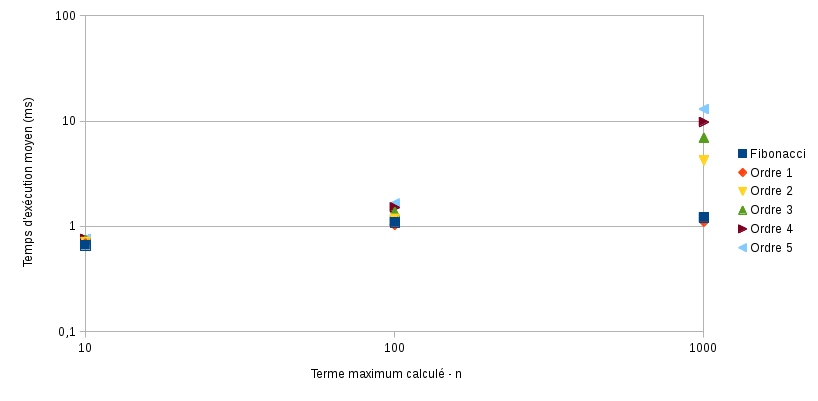
\includegraphics[scale=0.7]{figures/graphe.png}
            \caption{\label{fig:getitem}Rapport du temps de calcul avec \texttt{to\_list} sur le temps
            de calcul avec \texttt{forward\_matrix\_bsplit}, pour différentes valeurs de $n$, et différents
            ordres de récurrence. On utilise une échelle logarithmique.}
        \end{center} \end{figure}
        Ces résultats ont été obtenus en prennant la moyenne du temps d'exécution sur 10 exécutions avec
        des annihilateurs générés aléatoirement (et ne créant pas de singularité) et d'ordre fixé.
        On note que dès le 
        calcul d'éléments de l'ordre de $100$, la méthode \texttt{forward\_matrix\_bsplit} est déjà plus
        efficace. Notons également que l'influence de l'ordre de la récurrence semble augmenter pour 
        des valeurs plus élevées de $n$. 
        Ces résultats nous ont permis de déterminer empiriquement
        une valeur à partir de laquelle nous passons d'une méthode à l'autre. Nous avons fixé cette valeur
        a $100$.\\
        \par Le dernier point que nous avons implémenté concernant ces fonctions,
        est la possibilité d'utiliser les slices de Python. Les slices, sont des objets
        qui peuvent être paramètres de \texttt{\uline getitem\uline}. Pour une liste, ils permettent
        d'indiquer qu'on souhaite obtenir une \og tranche \fg\ de la liste, par exemple, les éléments
        8 à 13, éventuellement avec un pas. Dans notre cas, nous avons simplement adapté notre
        fonction, afin qu'elle calcule le premier élément de la tranche avec la méthode optimale,
        et les éléments suivants avec la méthode \texttt{to\_list} de l'annhilateur.


    \subsection{Structure d'anneaux : \texttt{\uline add\uline } et \texttt{\uline mul\uline}}
        \label{sec:ring}
        Nous avons déjà évoqué le fait que les suites P-récursives forment un anneau,
        l'implémentation des fonctions d'addition et de multiplication était donc une étape
        importante de l'avancée du projet.
        Il est facile de montrer que le plus petit commun multiple à gauche (\texttt{lclm})
        est un annihilateur de la somme de deux suites :
        soient $a_1$ et $a_2$, deux annihilateurs des suites $u_1$ et $u_2$ respectivement,
        et supposons que leur ppcm à gauche $a_{sum} = ba_1 = b'a_2$ existe. On a :
        \begin{align*}
            a_{sum}(u_1+u_2) &= a_{sum}u_1 + a_{sum}u_2\\
            &= ba_1u_1 + b'a_2u_2 = 0\quad \text{CQFD}
        \end{align*}

        La fonction qui calcule le plus petit commun multiple à gauche de deux suites
        est \texttt{lclm}, pour \textit{least common left multiple}, et est fournie par la
        bibliothèque \textsc{OreAlgebra}. 
        Si la nouvelle suite est d'odre $k$ alors ses conditons initales seront la somme des 
        $k$ premiers termes des deux suites. Pour cela nous utilisons la fonction
        \texttt{to\_list} que nous avons écrite
        et récuperons les $k$ premiers éléments des suites et les sommons.
        Par exemple si l'on ajoute la suite de \texttt{Fibonacci} et celle de \texttt{Tribonacci} :
        \begin{align*}
            \textnormal{Fibonacci : } &F_{n+2} - F_{n+1} - F_n = 0,\qquad F_0=0, F_1=1\\
            \textnormal{Tribonacci : } &T_{n+3} - T_{n+2} - T_{n+1} - T_n = 0,\qquad T_0 = 0, T_1 = 1, T_2 = 1\\
            \textnormal{Leur Sommme : } &S_{n+5} - 2S_{n+4} - S_{n+3} + S_{n+2} + 2S_{n+1} + S_n = 0,\\
            &S_0 = 0, S_1 = 2, S_2 = 2, S_3 = 4, S_4 = 7
        \end{align*} 
        
        \par Cependant la suite nouvellement formée peut présenter une ou plusieurs singularité.
        Prenons la cas
        de la somme des suites des  \texttt{Entier consecutif} et \texttt{Fibonacci}
        \begin{align*}
            \textnormal{Ent. Consec. : } &nE_{n+1} - (n+1)E_n = 0,\qquad E_0 = 0, E_1 = 1\\
            \textnormal{Fibonacci : } &F_{n+2} - F_{n+1} - F_n = 0,\qquad F_0=0, F_1=1\\
            \textnormal{Leur Sommme : } &(n - 1)D_{n+3} + (-2n + 1)D_{n+2} + D_{n+1} + nD_n = 0, \\
            &D_0 = 0, D_1 = 2, D_2 = 3\\
        \end{align*} 
        La somme est d'ordre 3, on devrait donc sommer les 3 premiers termes de E et F (respectivement 
        $(0,1,2)$ et $(0,1,1)$) ce qui donnerait comme conditions initiales pour D : $(0,2,3)$.
        Si 
        l'on essaie de dérouler la récurrence pour calculer le prochain terme, nous obtenons $D_3 = 5$,
        mais nous remarquons que le terme $D_4$ est singulier (cf section \ref{sec:cons}), et ne peut 
        être calculé. En revanche, $F_4$ et $E_4$ existent, nous avons donc décidé que lorsque l'annihilateur
        de la somme de deux suites est dans un cas similaire à celui-ci, nous calculons la somme des
        singularités et les rajoutons dans les conditions initales.
        \par En ce qui concerne la multiplication, le principe est exactement le même sauf que la 
        multiplication de deux opérateur se calcule grâce à la fonction \texttt{symmetric\_product},
        qui est également fournie par \textsc{OreAlgebra}.
        par exemple si l'on veux multiplier.\\
        %Pour ce qui est de la somme et multiplication de suite par une constante, cela est possible, mais 
        %note module ne respecte pas les principe de Sage sur la coercion.
        %\begin{align*}
        %    &R,n = ZZ["n"].objgen()\\
        %    &A,Sn = OreAlgebra(R,"Sn").objgen()\\
        %    &catalan = PRecSequence([1,1],(n + 2)*Sn - 4*n - 2)\\
        %    &pascal = PRecSequence([1,1],Sn**2 - Sn - 1)\\
        %    &s1 = pascal * catalan \qquad\# fonctionne\\
        %    &s2 = catalan + 2 \qquad\# fonctionne\\
        %    &s3 = 1 + catalan \qquad\# ne fonctionne pas\\
        %\end{align*} \\


    \subsection{Autres objectifs}
        En plus des objectifs principaux, nous avons rempli certains des autres objectifs.
        Par exemple, la possibilité d'utiliser d'autre anneaux que $\mathbb Z$ (sur lequel
        nous nous sommes concentrés pendant le développement) est venue, et de manière assez
        surprenante, "naturellement". Nous n'avons en effet eu pas ou peu à travailler
        spécifiquement en adaptant le code à $\mathbb Z$, et il fonctionne ainsi également
        pour $\mathbb Q $ et $\mathbb R $. Nous n'avons par contre pas essayé avec des anneaux
        dont la structure est plus compliquée comme $\mathbb C$ ou $\mathbb F_p$.\\
        \par En ce qui concerne la manipulation des suites constantes, nous avons avec
        succès implémenté la possibilité de changer le comportement du constructeur de la classe
        dans le cas où il reçoit une constante en paramètre. Nous avons également implémenter la
        possibilité de tester si une suite est constante, ce qui incidemment nous permet
        également de tester si deux suites sont égales. Il suffit en effet de faire la différence
        des deux suites, et tester si la différence est constante. Si c'est le cas, nous 
        vérifions que cette constante est 0.\\
        \par Enfin, la fonctionnalité de deviner la récurrence à partir des premiers
        termes d'une suite a simplement consister à un appel à la fonction \texttt{guess}
        de \textsc{OreAlgebra}.

\setcounter{secnumdepth}{0}
\section{Conclusion}
    Dans l'ensemble, nous avons réussi à développer une classe répondant aux objectifs
    principaux que nous nous étions fixés.
    Celle-ci permet une manipulation basique des suites P-récursives 
    et propose également des fonctionnalités secondaires, telle que la possibilité de travailler
    dans différents ensembles ($\mathbb{Z,Q,R}$, nous n'avons pas testé $\mathbb{C}$ et 
    $\mathbb F_p$), ou bien la manipulation de constantes comme une suite récursive.\\
    Les principales difficultés que nous avons rencontrées, ont été pour la plupart liées
    à des problèmes de définitions, ou de paradigme. Pour les contourner, il a fallu
    se mettre à la place de l'utilisateur du module, et comprendre ce qu'il en attend lorsqu'il choisit
    de l'utiliser. Certains dilemmes n'ont pas de solution unique, et dépendent du cas spécifique
    auquel est confronté l'utilisateur. Pour cette raison, nous nous sommes efforcés de rester 
    généraliste dans la manière dont nous traitions les problèmes, et de rendre les traitements
    spécifiques optionnels.\\
    \par Aujourd'hui le recul nous pouvons affirmer que nous aurions fait certaines choses
    différemment, ou d'autres choix
    comme par exemple la manière de traiter les singularités et les conditions
    initiales. Nous sommes cependant satisfaits du travail accompli dans l'ensemble.\\
    \par Concernant les perspectives d'ammélioration, il y a bien sur la complétion des objectifs
    encore non atteints, mais également la possibilité de se rapprocher des directives de
    développement de Sage. Il existe également un axe de généralisation et la systématisation
    de cette approche à d'autres objets vivant dans des algèbres d'Ore.\\
    \subsection*{Conclusions personnelles}
        \textbf{Aurélien} :
        Grâce à ce projet j'ai pu apprendre le côté orienté objet de Python que je n'avais jamais vu
        jusqu'à maintenant.
        De même j'ai appris à manipuler et me à servir SageMath et les fonctions du module 
        \textsc{OreAlgebra}. J'ai également pu appren à utiliser \LaTeX.\\[1cm]
        \par \textbf{Mathis} : Ce projet m'a permis de renforcer mes connaissances en Python.
        \c{C}a a également été l'occasion de se plonger dans un projet de grande ampleur.
        En lire le code, et apprendre à essayer de développer dans ce cadre sont des expériences qui,
        d'après moi, font le plus défaut aux étudiants en université.

\newpage
\bibliographystyle{abbrv}
\nocite{*}
\bibliography{PSFPN.bib}

        
       

%----------------------------------------------------------------------------------------



\end{document}


